\chapter{QDSP}
\section{Concept}
The basis of the design comes from the QDSP designed by Anders Steengaard. This design was maintained in the VHDL as to support interoperability between the old and new design while additional features were added. The overall design of the DSP can be seen in \figref{fig:DSPDiagram}. The design was created to allow the DSP to be inserted in applications that use $\mu$TosNet or UnityLink and only requre minimal changes to the existing VHDL. The result of this design is that the DSP has two main memory areas, on to interface with the surrounding vhdl, called the IO memory, and one to either $\mu$TosNet or Unity-Link refereed to as the Shared memory.

\begin{figure}[h]
	\centering
		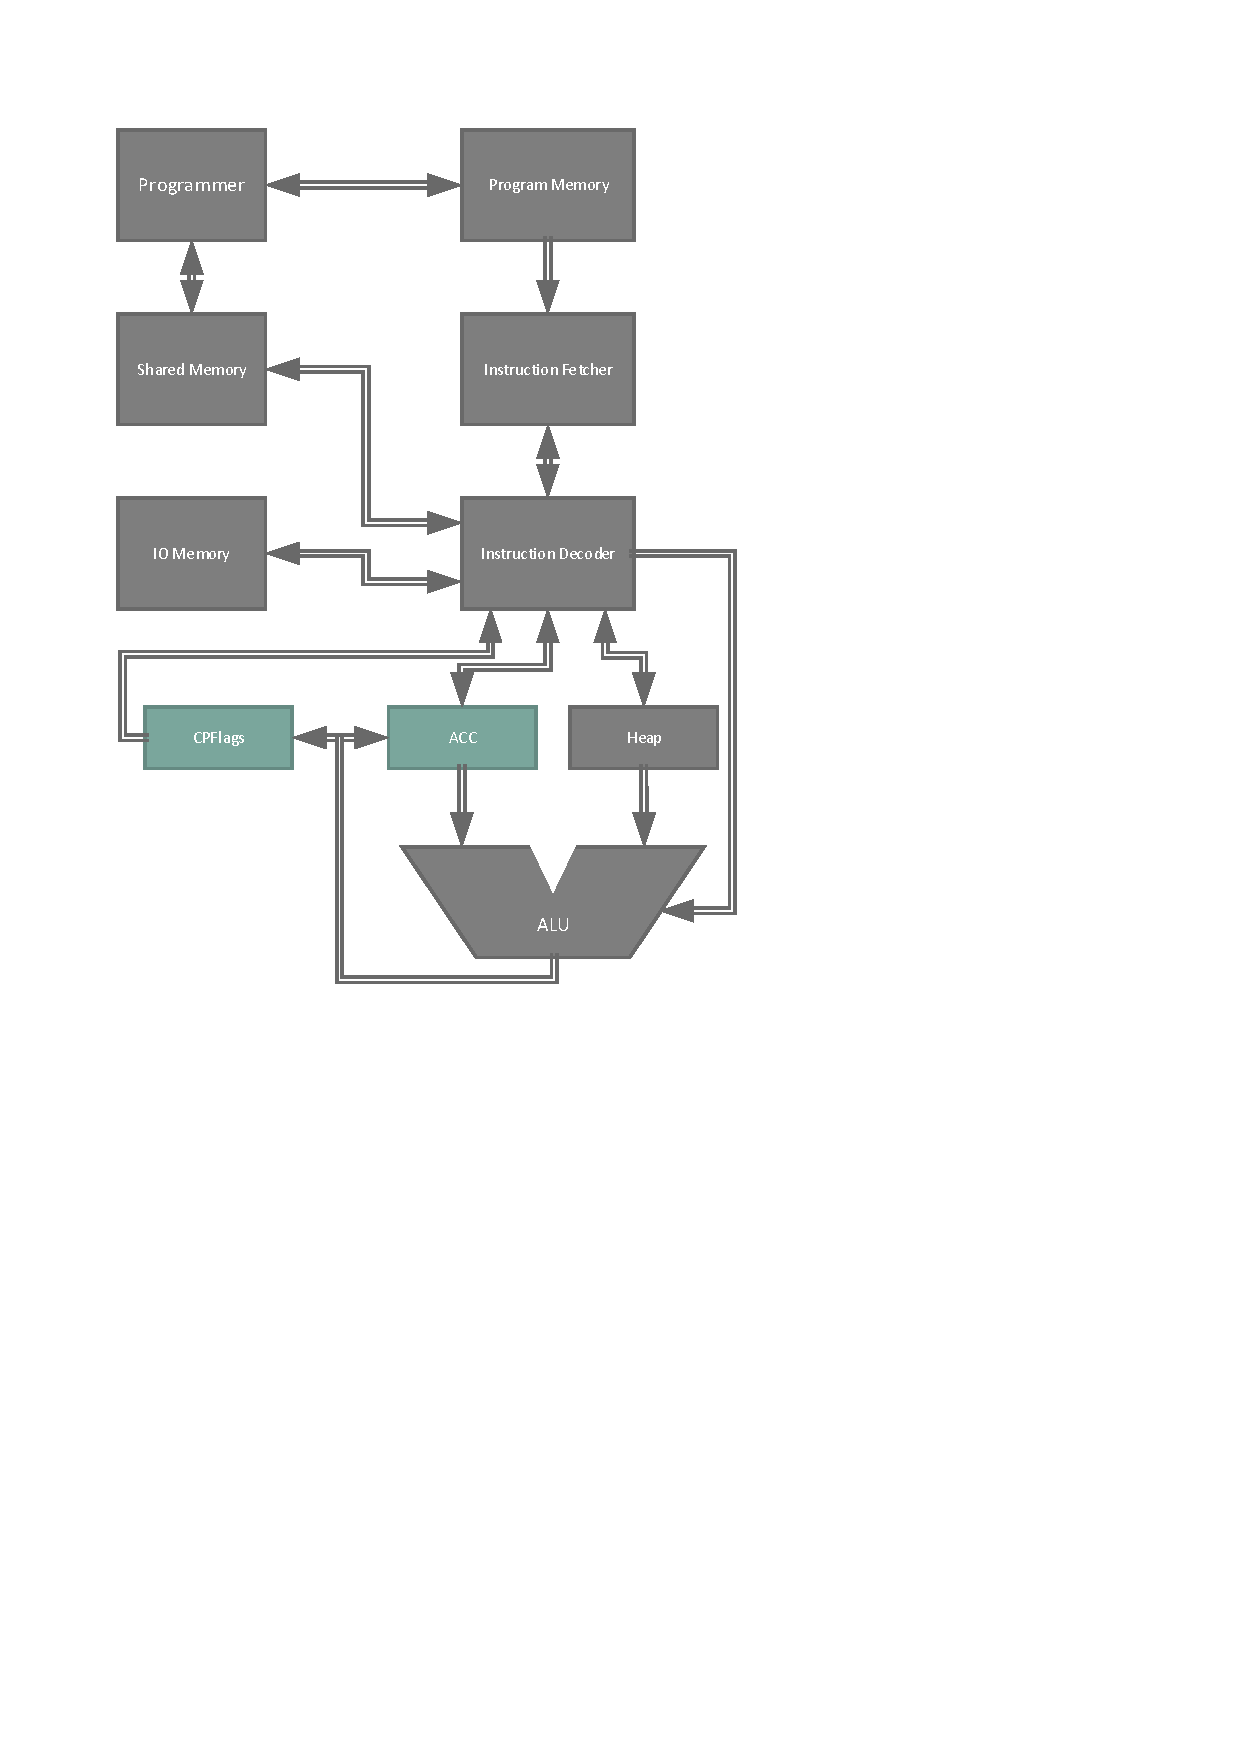
\includegraphics[width=0.40\textwidth]{../includes/pictures/DSPDiagram.pdf}
	\caption{Block diagram of QDSP}
	\label{fig:DSPDiagram}
\end{figure}

\section{Instructions}

The structure of the instruction-set from the original QDSP was designed to allow for arguments to be provided along with the instruction. This was done by having a fixed length instruction followed by argument, this structure was maintained in this new design.

The instruction-set was updated to allow for new features such as branching whereby evaluations on values could be made and subsequent jumps in the program code could be made, allowing for loops and conditional code execution.

The full instruction set available for the QDSP is seen in \tabref{tab:instruction-set}

\begin{table}[ht]
	\rowcolors{2}{table-gray}{}
	\centering
		\begin{tabular}{c|c|p{8cm}}
	\textbf{Name} & \textbf{Argument} & \textbf{Description} \\ \hline
	NOP & N/A & No Operation \\ 
	CAH & Heap address & Copy accumulator to heap\\ 
	CHA & Heap address & Copy heap value to accumulator\\ 
	RST & N/A & Reset program counter to 0 \\ 
	LDX & N/A & Test if program loader is requested on memory interface\\ 
	CAS & Memory address & Copy accumulator to shared memory \\ 
	CSA & Memory address & Copy shared memory value to accumulator \\ 
	CAI & Memory address & Copy accumulator to IO memory\\ 
	CIA & Memory address & Copy IO memory value to accumulator\\ 
	ADD & Heap address & Add Heap to accumulator \\ 
	SUB & Heap address & Subtract heap from Accumulator\\ 
	BDIV & Shift count & Signed binary division using bit shifting\\ 
	BMUL & Shift count & Signed binary multiplication using bit shifting\\ 
	MUL & Heap address & Multiply Heap with accumulator\\ 
	TRN & N/A & Truncate accumulator to 16bit value\\ 
	MAX & Heap address & Compares accumulator to heap value and set accumulator to the highest of the two\\ 
	MIN & Heap address & Compares accumulator to heap value and set accumulator to the smallest of the two\\ 
	LSH & Shift count & Left shifts accumulator the given amount\\ 
	RSH & Shift count & Right shifts accumulator the given amount\\ 
	JMP & Program memory address & Changes program counter to specified program memory address\\ 
	BRE & Program memory address & Changes program counter to specified program memory address, based on compare flags\\ 
	BRG & Program memory address & Changes program counter to specified program memory address, based on compare flags\\ 
	BRL & Program memory address & Changes program counter to specified program memory address, based on compare flags \\ 
	CMP & Heap address & Compares heap value with accumulator and set compare flags based on the results\\ 
\end{tabular}
	\caption{QDSP Instruction set}
	\label{tab:instruction-set}
\end{table}